\documentclass[conference]{IEEEtran}
\IEEEoverridecommandlockouts
% The preceding line is only needed to identify funding in the first footnote. If that is unneeded, please comment it out.
%Template version as of 6/27/2024

\usepackage{cite}
\usepackage{amsmath,amssymb,amsfonts}
\usepackage{algorithmic}
\usepackage{graphicx}
\usepackage{textcomp}
\usepackage[dvipsnames]{xcolor}
\usepackage{url}
\usepackage{mathtools}
\usepackage{relsize}
\usepackage{amsmath}
\usepackage{amssymb}
\usepackage{amsfonts}
\usepackage{tikz}
\usetikzlibrary{decorations.pathreplacing}
\usetikzlibrary{arrows.meta}

%\def\BibTeX{{\rm B\kern-.05em{\sc i\kern-.025em b}\kern-.08em
%    T\kern-.1667em\lower.7ex\hbox{E}\kern-.125emX}}

\DeclareUrlCommand\email{\urlstyle{tt}}
\DeclareUrlCommand\website{\urlstyle{same}}
\DeclareUrlCommand\directory{\urlstyle{same}}
\newcommand{\hash}{{\mathit{hash}}}
\newcommand{\difficulty}{{\mathit{difficulty}}}
\newcommand{\delay}{{\mathit{delay}}}

\colorlet{lightred}{red!50!white}
\colorlet{verylightgray}{gray!25!white}

\newcommand{\computer}{\includegraphics[width=1.3cm]{pictures/computer}}
\newcommand{\leftArrow}{\includegraphics[width=0.6cm]{pictures/left_arrow}}
\newcommand{\signature}{\includegraphics[width=0.3cm]{pictures/signature}}
\newcommand{\leftplug}{\includegraphics[width=0.7cm]{pictures/plug_left}}
\newcommand{\rightplug}{\includegraphics[width=0.7cm]{pictures/plug_right}}
\newcommand{\ssd}{\includegraphics[width=0.8cm]{pictures/ssd}}

\begin{document}

\title{Mobile Mining for Proof of Space}
%\thanks{Thank funding institutions, if any.}

\author{\IEEEauthorblockN{1\textsuperscript{st} Given Name Surname}
\IEEEauthorblockA{\textit{dept. name of organization (of Aff.)} \\
\textit{name of organization (of Aff.)}\\
City, Country \\
email address or ORCID}
\and
\IEEEauthorblockN{2\textsuperscript{nd} Given Name Surname}
\IEEEauthorblockA{\textit{dept. name of organization (of Aff.)} \\
\textit{name of organization (of Aff.)}\\
City, Country \\
email address or ORCID}
\and
\IEEEauthorblockN{3\textsuperscript{rd} Given Name Surname}
\IEEEauthorblockA{\textit{dept. name of organization (of Aff.)} \\
\textit{name of organization (of Aff.)}\\
City, Country \\
email address or ORCID}
\and
\IEEEauthorblockN{4\textsuperscript{th} Given Name Surname}
\IEEEauthorblockA{\textit{dept. name of organization (of Aff.)} \\
\textit{name of organization (of Aff.)}\\
City, Country \\
email address or ORCID}
\and
\IEEEauthorblockN{5\textsuperscript{th} Given Name Surname}
\IEEEauthorblockA{\textit{dept. name of organization (of Aff.)} \\
\textit{name of organization (of Aff.)}\\
City, Country \\
email address or ORCID}
\and
\IEEEauthorblockN{6\textsuperscript{th} Given Name Surname}
\IEEEauthorblockA{\textit{dept. name of organization (of Aff.)} \\
\textit{name of organization (of Aff.)}\\
City, Country \\
email address or ORCID}
}

\maketitle

\begin{abstract}
The abstract goes here.
\end{abstract}

\begin{IEEEkeywords}
blockchain, proof of space, mining, mobile mining, energy consumption.
\end{IEEEkeywords}

\section{Introduction}\label{sec:introduction}

Blockchain is a distributed network of computers (\emph{peers}).
Each peer receives transaction requests, that eventually packs
into new \emph{blocks}. These form a growing tree,
with each block pointing back to the previous one. Mining is the process of
block creation and includes a notion of chain quality that
decides which of the many tree branches eventually emerges
as the stable chain, on which all peers agree,
therefore reaching \emph{consensus}. Mining
is normally remunerated: the block creator has the right to
mint and earn a predetermined amount of cryptocurrency for each block that it creates.
%as well as to earn a small fee on the transactions included in the blocks.

This very abstract description is explicitly generic \wrt{} two implementation choices:
%
\begin{enumerate}
  \item The notion of transaction. This is irrelevant in this paper.
    In general, a transaction is the specification of an
    operation whose execution modifies the state of an abstract machine.
    For instance, a money transfer
    in Bitcoin~\cite{Nakamoto08} or
    the execution of some code over a shared state of objects
    in Ethereum~\cite{AntonopoulosW25}
    (and in other blockchains that support Turing-complete smart contracts,
    up to gas exhaustion).
  \item The mining algorithm. Namely, Bitcoin pioneered the
    proof of work algorihtm~\cite{DworkN92}, while more modern blockchains tend to use a
    proof of stake algorithm~\cite{Kwon14}, and this paper focuses on a proof
    of space algorithm~\cite{Spoto25}.
\end{enumerate}

In Bitcoin's proof of work,
minted blocks carry evidence of the performance of some computational
work for their creation. The more this work, the higher the
likelihood for the blocks to be integrated in the stable chain of the blockchain.
It is well-known that this generates high electricity costs for CPU
computation and data centers, with a high ecological impact (resource
consumption, e-waste). Moreover, this induces the concentration of mining power in countries
where electricity is cheap, against the idea of full decentralization.

The proof of stake approach emerged as a reaction to this. Its idea is that
only a restricted set of peers (\emph{validators}) can mint blocks.
This makes mining cheaper, efficient and ecologically sustainable.
Non-validators can stake on the success of validators, which introduces some form
of decentralization, but
it is generally accepted that proof of stake is more centralized than proof of work.
Nevertheless, it is the most used mining algorithm at the moment.

Proof of space is a less-known family of
algorithms~\cite{AbusalahACKPR17,AtenieseBFG14,CohenP19,DziembowskiFKP15,ParkKFGAP18,RenD16,Spoto25}.
Its idea is that minted blocks carry evidence
of the allocation of a large data structure on disk for their creation.
The larger this structure, the higher the likelihood that
such blocks get included in the stable chain. Proof of space is decentralized like
Bitcoin's proof of work and ecologically sustainable like proof of stake, although the actual
disk degradation (e-waste), due to mining, has not been studied up to now.

This paper focuses on \emph{mobile mining}, that is,
mining on a mobile phone or tablet. In principle, this is appealing because:
%
\begin{itemize}
\item it leverages a huge existing hardware base of devices, that otherwise remain idle
  for most of the time;
\item it introduces mining to a large portion of humanity, who owns a
  phone but not a powerful connected computer;
\item it can be easily updated, thanks to the automatic update system of mobile phones;
\item it simplifies the start-up of new blockchains, since it is easier to convince people
  to install an app than to run and maintain a software on an always connected computer.
\end{itemize}
%
Mobile mining has not been used up to now because of obvious limitations
of mobile phones \wrt{} battery capacity and network bandwidth, in particular
in least favorite countries.
%This paper shows that
%proof of space emerges as a niche solution here, whose mining
%is less sensitive to these limitations.

This paper makes the following contributions:
%
\begin{enumerate}
\item it presents mobile mining, its power and limitations;
\item it shows how proof of space emerges as a niche solution here, whose mining
  is less sensitive to these limitations;
\item it presents Mokaminter, our actual Android app for mobile mining with proof of space;
\item it reports experiments with Mokaminter, discussing its battery consumption
  and amount of exchanged data.
\end{enumerate}
%
It must be clear that Mokaminter runs only a miner in the phone, not a full blockchain
peer, which would be prohibitive for many reasons, such as the size of the blockchain,
that of its state database, the amount of data exchanged and the computational
cost. The blockchain peer is assumed to be an external computer, that the miner contacts
from the phone.

The rest of this paper is organized as follows.
Sec.~\ref{sec:related_work} discusses related work.
Sec.~\ref{sec:mining} gives a uniform description of various mining algorithms.
Sec.~\ref{sec:remote_mining} considers if such algorithms can be implemented
on a mobile phone, connected to a blockchain peer.
Sec.~\ref{sec:mokaminter} presents the Mokaminter mobile app for mining
with proof of space.
Sec.~\ref{sec:experiments} confirms Mokaminter's low battery consumption
and reduced exchanged data.
Sec.~\ref{sec:conclusion} concludes.

\section{Related Work}\label{sec:related_work}

Proof of space is a mining algorithm where disk (currently SSD) space
is used instead of CPU power.
It is energetically more efficient than proof of work and
more decentralized than proof of stake.
A preliminary
\emph{plotting phase}, when large data is allocated on disk,
through a potentially expensive process, is followed by a
\emph{mining phase}, when such data is used to quickly answer
block creation challenges received from blockchain peers:
the probability to create blocks for the stable chain
is proportional to the size of the allocated disk space.

Pioneering work~\cite{AtenieseBFG14,DziembowskiFKP15} introduced
formal proofs on persistent storage, showing that
CPU-bound on-demand recomputations (or \emph{replotting attacks}~\cite{BaigGP25}) are not viable,
due to high complexity pebbling graphs and Merkle trees:
any attempt to reduce the allocated space adds a prohibitive recomputation cost.
A subsequent evolution~\cite{RenD16}
uses \emph{stacked expanders} to reduce the implementation cost
and simplify proofs. The SpaceMint prototype~\cite{ParkKFGAP18},
now discontinued, showed the approach feasible and considered
mitigations to potential attacks, typical of
proof of space, such as mining on multiple chains or block/challenge grinding.
Chia~\cite{AbusalahACKPR17,CohenP19}, a more robust implementation, combines
space with verifiable delay functions, in a hybrid proof of space and time mechanism.
In Filecoin~\cite{Fil24}, parties commit space and show, repeatedly,
that they are still storing data in the committed space.
%While Chia is fully-permissionless, Filecoin is
%quasi-permissionless: anybody can participate, but under some requirements.
We build on the proof of space algorithm of Signum~\cite{signum},
previously Burstcoin, based on the precomputation of
plot files that later support quick block creation, as formalized
in~\cite{Spoto25}. Plot file are too expensive to recreate
on-the-fly for each block. We work with the generic blockchain
engine Mokamint~\cite{mokamint}, derived from Signum's algorithm, but generic \wrt{} the
notion of transactions, delegated to an application layer over Mokamint.

There is a lack of scientific research on the use of mobile phones for blockchain mining.
In~\cite{LeePSB20}, a blockchain system is proposed, to build local
industrial IoT blockchain networks, where drones are mobile miners
based on proof of work. This does not scale
to a global blockchain and to mobile phones, that
are not competitive against expensive specialized hardware and whose battery
would immediately get drained by the proof of work.
The same consideration applies to~\cite{SuankaewmaneeHN18}, that
presents a specialized blockchain for mobile commerce, with Android phones as
mobile miners based on proof of work.
Experiments are reported for blocks holding up to six transactions,
which is sensible for a local blockchain but irrealistic for a global one.
Despite its title, \cite{JiangLW22}~tackles a different problem, namely,
how to offload blockchain applications
to a cloud computing provider to make them usable
with the limited resources of the phone.
More generally, this approach allows edge devices, with strong hardware limitations,
to offload computationally expensive
tasks to external servers and to the cloud~\cite{SoundararajS25}.
The goal of the present paper is instead to perform mining \emph{in} the mobile phone
and offload the mining process from blockchain peers to many
mobile phones, expected to run a mobile mining app.

A simple search on Google Play reports a few Android apps for
\emph{crypto mining}. A deeper look makes it clear that,
despite their name, these apps are not miners, but
fall in either of the following categories.
(1) Mobile dashboards
    to cloud pool miners: mining occurs in the cloud and
    the app is just monitoring.
    This is the case, for instance, of Ct Pool~\cite{ctpool-google-play},
    ViaBTC~\cite{viabtc-google-play},
    ECOS~\cite{ecos-google-play},
    Cloud Mining Bitcoin Crypto~\cite{cloudminingbitcoincrypto-google-play}
    and MineX~\cite{minex-google-play}.
(2) Dubious games that promise Bitcoins in exchange of solving tasks
    or watching ads. This is the case, for instance,
    of Bitcoin Miner Earn Real Crypto~\cite{bitcoinminerearnrealcrypto-google-play}
    and Crypto Fortune Tycoon: BTCMiner~\cite{cryptofortunetycoonbtcminer-google-play}.
In particular, our research did not find any app for actually mining \emph{in} a phone.

\section{An Abstract Presentation of Mining}\label{sec:mining}

The different mining algorithms can be actually presented
inside a uniform setting. Namely, mining is a competitive game,
played, concurrently and independently, by each peer of a blockchain network.
Its goal is to choose which peer wins the right to create the \textbf{next}
block of the blockchain. This block must be \emph{valid}, that is, respect
all consensus rules, that are largely blockchain-specific. For example,
\textbf{next} must point back to the previous top of the blockchain; and
the transactions included in \textbf{next} must have valid signatures. But the
actual list of consensus rules is quite larger.

Mining algorithms can be presented in terms of:
%
\begin{itemize}
\item \emph{challenge}: given the current chain $\xi$,
  determine, deterministically,
  a challenge for \textbf{next};
\item \emph{answer}: create, if possible,
  a \textbf{next} that satisfies the challenge;
\item \emph{competition}: in case of more possible \textbf{next}, prefer the \emph{best}
  one \textit{wrt.\ }some notion of chain quality.
\end{itemize}
%
Each peer performs the mining algorithm, whispers the resulting \textbf{next} block to its
connected peers and receives the \textbf{next} block of its connected peers. In case
of more alternatives for \textbf{next}, the competition rule is used to choose the
emerging winner. This gives rise to a \emph{consensus algorithm}, which uses the mining
algorithm as a subroutine.

For proof of work, the general scheme for the mining algorithm becomes:
%
\begin{itemize}
\item \emph{challenge}: compute an integer $\difficulty$ from $\xi$
  and find a valid \textbf{next} such that
  $\hash(\mathbf{next})\ge\difficulty$;
\item \emph{answer}: create a \textbf{next} by rotating among possible
  values for its nonce field, until $\hash(\textbf{next})\ge\difficulty$;
\item in case of more possible \textbf{next}, prefer that with the largest hash.
\end{itemize}
%
The algorithm for computing $\difficulty$ is not relevant here.
Moreover, note that Bitcoin's proof of work is traditionally specified
in terms of the \emph{smallest} hash, but we prefer the equivalent
definition above, in terms of the largest hash,
to match the intuition that a higher $\difficulty$ makes mining harder.

For proof of stake, the generally accepted idea is that there is
\emph{no} mining~\cite{Kwon14}. However, a mining algorithm can be defined
also in this case:
%
\begin{itemize}
\item \emph{challenge}: compute an integer $i$ from $\xi$ (the index of the chosen
  validator) and find a valid \textbf{next};
\item \emph{answer}: if this algorithm is run by the $i$th validator,
  create a valid \textbf{next} block; otherwise, do not create any \textbf{next};
\item in case of more possible \textbf{next}, choose any of them, since
  the choice is irrelevant for what mining is concerned.
\end{itemize}
%
The algorithm for computing $i$ is irrelevat here: usually, a simple
round-robin is used. Moreover, what is reported above is the mining
algorithm, not the consensus algorithm, that is typically based on a Byzantine
protocol of pre-votes and pre-commits~\cite{Kwon14}.

Finally, proof of space, as presented in~\cite{Spoto25},
is based on the idea that \textbf{next} must contain
a data structure, called \emph{nonce}, that can be quickly recovered from disk from a
set of precomputed nonces (called, a \emph{plot file}). The mining algorithm in this case
becomes:
%
\begin{itemize}
\item \emph{challenge}: compute some data $\kappa$ from $\xi$;
\item \emph{answer}: create a valid \textbf{next} block, containing a nonce $\nu$
  from the plot file;
\item in case of more possible \textbf{next}, choose that with the smallest
  $\delay(\nu,\kappa)$ for its nonce $\nu$.
\end{itemize}
%
The algorithm for computing the challenge $\kappa$ is irrelevant here. In any case,
this $\kappa$ is used to choose a nonce from the plot file, whose quality measure,
the inverse of $\delay$, is maximized. The key point of this proof of space algorithm
is that the computation of the nonces (\emph{ie.}, of the plot file) is so expensive
that it cannot be done on-the-fly, at each mined block, but the plot file must be computed
instead once and for all, before starting mining, and kept on disk to answer, quickly, the mining
challenges. The consensus algorithm will use $\delay$ to wait for the time after which the block
becomes valid.

This abstract presentation of mining has the nice property of making it clear
that mining is a subroutine whose input is the challenge derived from the current
chain $\xi$ and whose output is the information needed to create \textbf{next}:
a nonce for proof of work and proof of space\footnote{Although the notion of nonce is
different in the two cases.}, and a Boolean for proof of stake
(create the block or rather let another validator create the block). As such, the
mining algorithm could be offloaded to a device external to the peer that holds
the blockchain and that creates \textbf{next}, as discussed in the next section.

\section{Remote Mining on a Mobile Phone}\label{sec:remote_mining}

It is natural to move the two software parts in
Fig.~\ref{fig:local_mining} into two distinct machines, connected by a network.
This is because many users want to run a miner on their machine, and earn cryptos,
but only a few are typically interested in running a full blockchain peer on their machine.
This is shown in Fig.~\ref{fig:remote_mining}, where connections in code
are replaced by network connections.

\begin{figure}[b]
  \begin{center}
    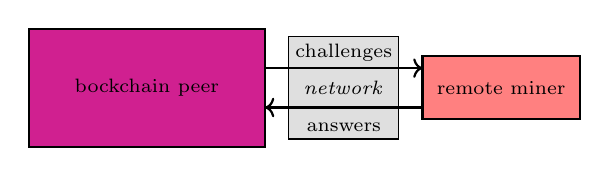
\begin{tikzpicture}
      \draw [fill=VioletRed,thick] (0,0) rectangle +(3,1.5);
      \draw (1.5,0.75) node {{\scriptsize bockchain peer}};

      \draw [fill=lightred,thick] (5,0.35) rectangle +(2,0.8);
      \draw (6.0,0.75) node {{\scriptsize remote miner}};

      \draw [fill=verylightgray] (3.3,0.1) rectangle +(1.4,1.3);

      \draw[->, thick] (3,1.0) -- (5,1.0);
      \draw (4.0,1.2) node {{\scriptsize challenges}};

      \draw[<-, thick] (3,0.5) -- (5,0.5);
      \draw (4.0,0.25) node {{\scriptsize answers}};

      \draw (4.0,0.75) node {{\scriptsize\emph{network}}};

    \end{tikzpicture}
  \end{center}
  \caption{Peer and remote miner connected through a network.}\label{fig:remote_mining}
\end{figure}

However, this graphically simple modification might result useless or impractical,
depending on the specific characteristics of the mining algorithm and of the machine
where the remote miner must be run. Let us consider, in particular, the case when this
machine is a mobile phone.

\subsubsection*{Proof of work}

In this case, the challenge must include the full block that is being
created, since the nonce must be chosen in a way that maximizes the block's hash.
For Bitcoin, a block size can be up to 1~MB, or even 4~MB after the Segregated Witness upgrade.
This data must be exchanged at the creation of each block, which is hard in many
countries, where mobile internet is slow; moreover, most operators fix a maximum number of
GB exchange in the month, which would be easily exhausted; finally, the computational cost
of proof of work would drain the telephone's battery. These considerations are enough
to conclude that, at the moment, mining for proof of space, for a global blockchain like
Bitcoin, on a mobile phone, remains irrealistic.

\subsubsection*{Proof of stake}

In this case, mining is limited to the validators and is very cheap.
The exchanged data between peer and miner is very limited.
However, there is no reason for the validators to offload their very simple mining activity.
Therefore, mining on a mobile phone is theoretically possible for proof of stake, but it does
not seem to be of any practical interest.

\subsubsection*{Proof of space}

In this last case, mining requires the use of disk space, but not the use of significant
CPU power. At the time of this writing, mobile phones have an average disk space
of 256~GB. This is smaller than the average 1000~GB of desktop computers, but still significant.
Moreover, the proof of space of~\cite{Spoto25} uses very small challenges (around 64 bytes)
and answers (nonces, compacted into \emph{deadlines} of around 200 bytes~\cite{Spoto25}).
In particular, the block being created is not needed for mining. This makes this proof
of space algorithm an ideal choice for a remote miner running on a mobile phone:
no need of significant CPU power, enough disk space on the phone and little data exchanged
with the peer. This is why it has been the choice for the implementation of our
Mokaminter app.

\section{The Mokaminter App}\label{sec:mokaminter}

We have developed the Mokaminter app for mining with proof of space.
It creates and maintains a list of remote miners, each connected
to a peer of the same or of different blockchains.
Mokaminter is an open-source app for Android, distributed
on Google Play~\cite{mokaminter-google-play} under
the Apache 2.0 license. Its source code is available from~\cite{mokaminter-source-code}.
An iPhone version might be available eventually,
but it is difficult to create since
it cannot leverage existing Java libraries from desktop miners.

Mokaminter works for blockchains built through
the Mokamint generic engine~\cite{mokamint}, that implements
the proof of space algorithm in~\cite{Spoto25}. Mokamint
implements the networking and consensus layers of
a blockchain, while the application layer is left generic and can be
built on top of Mokamint.
This idea of a pluggable application layer has been borrowed from Tendermint~\cite{Kwon14}.
Currently, the Hotmoka software~\cite{hotmoka}
for running smart contracts in a subset of Java~\cite{Spoto19}
is available as an application
of Mokamint. Therefore Mokaminter mines, at the moment,
for a blockchain with smart contracts in Java whose consensus is based
on proof of space, but it might mine for other blockchains in the future.

Creation and activation of a miner works as follows:
(1) the user specifies the URI (universal resource identifier) of a
  blockchain peer running Mokamint and the desired dimension of the plot file;
  %(Fig.~\ref{fig:mokaminter_add_miner}, above);
(2) the app creates a new private/public key pair to identify the miner,
  represented, as usual from Bitcoin's time~\cite{Antonopoulos23},
  in terms of a $12$ words mnemonics; % (Fig.~\ref{fig:mokaminter_add_miner}, below);
  alternatively, the user can insert the $12$ words of an existing key pair;
(3) the app informs the user about the expected size of the plot file
  and asks for confirmation; % (Fig.~\ref{fig:mokaminter_confirmation});
(4) if confirmed, the creation of the plot file starts in the background;
(5) once the plot file is created, the app adds a miner tile
  and activates a background process that mines by using the new plot file.
  %(Fig.~\ref{fig:mokaminter_mining}).

%\begin{figure}[t]
%  \begin{center}
%    \includegraphics[width=\textwidth/3]{pictures/mokaminter_add_miner}
%  \end{center}
%  \caption{Specification of the parameters for the creation of a miner.}
%  \label{fig:mokaminter_add_miner}
%\end{figure}

%\begin{figure}[b]
%  \begin{center}
%    \includegraphics[width=\textwidth/3]{pictures/mokaminter_confirmation}
%  \end{center}
%  \caption{Confirmation is required before creating a new plot file.}
%  \label{fig:mokaminter_confirmation}
%\end{figure}

%\begin{figure}[t]
%  \begin{center}
%    \includegraphics[width=\textwidth/3]{pictures/mokaminter_mining}
%  \end{center}
%  \caption{A new tile for a miner, working in the background. Eventually, its
%  cryptocurrency balance will increase.}
%  \label{fig:mokaminter_mining}
%\end{figure}

\subsubsection*{Security Considerations}
%
A lost or stolen phone is a relatively frequent event.
If the private key of the miner were kept in the phone, who finds
or steals the phone could also steal the cryptocurrency accumulated while mining.
Therefore, Mokaminter has been designed to avoid storing private keys in the phone.
Namely, after creating or importing the private/public key pair,
%(Fig.~\ref{fig:mokaminter_add_miner}),
only the public key is needed for creating the plot and for mining, and
the app forgets the private key. On the negative side, this means
that the user must not lose the $12$ words of the key pair,
or otherwise access to the earned cryptocurrency becomes impossible.

\subsubsection*{Usability Considerations}
%
A mobile app has quite different usability considerations
than a desktop application.
%
A first one is about feedback.
In a desktop application, the user could check warnings, error messages and logs.
In a mobile app, this is possible
but uncomfortable for most users. Therefore, Mokaminter gives feedback through
a heartbeat graphical effect that informs the user that it is
actually mining, producing nonces. Moreover, network disconnection
turns the miner's tile gray in the list of miners.
%
Another usability issue is related to the insertion of the
$12$ words, to import and existing key pair.
This is frustrating and error-prone in a mobile phone, through a software keyboard.
Thus, Mokaminter suggests the possible words while typing and the user can
autocomplete them.
%
A last issue is the risk of specifying a plot dimension that is
too large to complete the plot's creation in a reasonable time:
this would hang the phone and drain its battery. To avoid this risk,
Mokaminter imposes a maximum plot dimension, that can only be
overridden by an explicit choice of the user.

\subsubsection*{Technical Considerations}
%
Mokaminter uses websockets for network connections,
that perfectly match the continuous, bidirectional flow of challenges
and answers (Fig.~\ref{fig:remote_mining}). But network connection in a
mobile phone is less reliable than in a desktop computer, since
it gets frequently lost (thick walls, tunnels, network switches).
Mokaminter automatically tries to reconnect when the connection is lost or
no challenges have been received for an extended period of time. If it fails, it
tries again after a minute, to avoid draining the battery with
very frequent reconnection attempts.
%
Another technical issue is related to the background task for mining.
The Android system is extremely restrictive with background
tasks, since they might drain the battery. There are official guidelines
for them, but they changed across different Android versions and
phone manufacturers often add extra constraints. Many phones
turn Mokaminter off overnight, when
the Android system enters a special \emph{doze mode}. If this happens, it is enough
for the user
to turn it on again in the morning. A better solution does not seem in sight, at the moment.


\section{Experimental Results}\label{sec:experimental_results}

This section reports experiments with Mokaminter and measures
the main quality metrics for the app: the amount of data exchanged
and the percentage of CPU used for mining. If these were too high,
Mokaminter would not be usable.

\section{Conclusion}\label{sec:conclusion}

Talk about e-waste. No Mokaminter for iPhone. Limit of mobile mining once a new blockchain become mainstream.


\section*{Acknowledgment}

\bibliographystyle{IEEEtran}

\bibliography{biblio}

\end{document}
